Formally evaluating the effectiveness of a meta-toolkit for visual analytics is complex. Arguably the most convincing method would require two groups of programmers of equivalent skills to implement the same set of visual analytics programs with and without Obvious. Then, a judgment could be made from the time spent and the quality of the results. This methodology has been used to assess the InfoVis Toolkit [4] with students but is impractical for real Visual Analytics applications that are more complex and would not fit the scope of student projects.

Another method, used to validate Prefuse [3] would be to re-implement complex Visual Analytics applications using Obvious and assess the results, again in term of time and quality. This is what we have done and we report on our results here.

\subsection{Coding applications with Obvious}

This section shows how Obvious can implement common applications in information visualization such as the creation of a scatterplot or of a graph visualization. These examples explain how to combine obvious component to build an application, how to create data structure and spot patterns to use. The first usecase concerns the coding of a graph visualization with Obvious InfoVis Toolkit implementation and the second one based on the coding of a scatterplot by combining component from different Obvious implementations.

For both examples and in fact every creation of an Obvious application, developpers have to follow the following steps:

\begin{itemize}
 \item creation of an Obvious data structure directly with a constructor or through a factory. Three ways exist to fill the data structure:
 \begin{enumerate}
  \item wrapping an existing data structure from a targeted toolkit as shown in the first example
  \item using an Obvious reader to load an Obvious structure from a well known file format (CSV, GraphML...) as shown in the second example
  \item using Obvious methods to directly manipulate the data structure (addRow, addNode, addEdge...), this is not shown in both examples 
 \end{enumerate}
 \item creation of an Obvious visualization with the created data structure and a map of parameters directly with a constructor or through a factory
 \begin{enumerate}
  \item as shown in the second example, it is possible to combine data structure from one Obvious implementation with visualization from another Obvious implementation
  \item the map parameter allows developpers to customize the Obvious monolithic component (in the second example, the map indicates columns used for X and Y axis of the scatterplot)
 \end{enumerate}
 \item creation of an Obvious view with the created visualization directly with a constructor or through a factory
\end{itemize} 

\lstset{frame=single,columns=flexible,numbers=left,numberstyle=\tiny,basicstyle=\small,language=Java,caption={Visualizing a graph with Obvious},label=codeSample1}
\begin{lstlisting}
// Creates the graph structure. First, set the factory to use (ivtk).
// Then load the native data structure, and get a factory instance.
// Finally, call the convenient getter of the factory.
System.setProperty("obvious.DataFactory",
    "obvious.ivtk.data.IvtkDataFactory");
infovis.Graph g = Algorithms.getGridGraph(10, 10);
DataFactory factory = DataFactory.getInstance()
Network network = factory.createGraph(g);

// Creates the associated visualization using the
// factory for visualization. No predicate and extra
// parameters are given to the constructor.
Visualization vis = new IvtkVisualizationFactory()
    .createVisualization(network, null, "network", null);

// Creates the view. No predicates and extra parameters are given to
// the constructor.
View view = new IvtkObviousView(vis, null, "graphview", null);
// Standard Java window creation
JFrame frame = new JFrame();
JScrollPane panel = new JScrollPane(view.getViewJComponent());
frame.add(panel);
frame.pack();
frame.setVisible(true);
\end{lstlisting}

\lstset{frame=single,columns=flexible,numbers=left,numberstyle=\tiny,basicstyle=\small,language=Java,caption={Combining different Obvious implementations to display a scatterplot},label=codeSample2}
\begin{lstlisting}
// Defining the data factory to use,
// obvious-prefuse will be used for the data structures.
System.setProperty("obvious.DataFactory",
    "obvious.prefuse.PrefuseDataFactory");
// Creating an Obvious CSV reader and loading an
// Obvious table
CSVImport csv = new CSVImport(new File("example.csv"), ',');
Table table = csv.loadTable();

// Creating the parameter map for the monolithic object.
Map<String, Object> param = new HashMap<String, Object>();
param.put(IvtkScatterPlotVis.X_AXIS, "id"); // xfield
param.put(IvtkScatterPlotVis.Y_AXIS, "age"); // yfield

// Creating the visualization then the view. No predicates are given to
// the constructor.
Visualization vis = new IvtkScatterPlotVis(table, null, "plot", param);

View view = new IvtkObviousView(vis,  null, "plot", null);
// Standard Java window creation
...
\end{lstlisting}

\subsection{Example using Weka}

Weka \cite{Weka} is a suite of machine learning software widely used to design applications particularly for visual analytics \pierreluc{I should put a reference here to justify this affirmation. Can you suggest one?}. Thus, Obvious in its obviousx package supports mechanisms to build Instances (main data structure of Weka) from Obvious Table. Several methods exist to link an Obvious structure with a Weka one:

\begin{itemize}
\item an Obvious table can be loaded into a Weka Instances. Since "Instances" is a data structure specially optimized for fast processing with clustering and machine learning algorithms, with this approach the developer benefits from Weka optimizations in terms of execution time.
\item an Obvious table can wrap a Weka Instances: Obvious tables translates its methods to Weka ones. With this approach, data are not duplicated in memory.
\end{itemize}

Both methods are equivalent in terms of lines of code and can be completed with the same machine learning algorithms from Weka. For instance, to wrap an existing table into a weka Instances, developpers simply need to add the following line to the code sample \ref{codeSample2} :

\lstset{frame=single,columns=flexible,numbers=left,numberstyle=\tiny,basicstyle=\small,language=Java,caption={Wrapping an Obvious Table into Weka Instances},label=wekaExample}
\begin{lstlisting}
Instances inst = new ObviousWekaInstances(table, "Instances");
\end{lstlisting}

To wrap the Obvious structure, the constructor simply needs as argument the Obvious table and a name for the weka Instances. Then, developpers can apply to this new Instances all machine learning algorithms defined in Weka. Creating this wrapper takes less than a week for one developper knowing well Obvious but discovering Weka.

This example demonstrates an important gain of Obvious: when a toolkit adopts Obvious it can immediately benefit from existing wrappers to complementaries functionalities. Thus, with the obviousx.weka package, all Obvious implementations can now provide advanced machine learning capabilities to their users.

\subsection{EdiDuplicate (a DDupe-Like application)}

INRIA maintains a database for the publications of its member. Researchers regularly fill this database, called HALINRIA, with their new publications. However, mistakes often appear during this process: duplicated authors or institutions or papers. Thus, in order to increase data consistency, INRIA is interested in a tool that can detect potential duplicates and use information visualization techniques to help the database administrator to merge duplicated items. An existing application, DDupe, already handles those tasks, but since it can not work directly with a database, we decide to use Obvious to build this tool, called EdiDuplicate.

Concretely, DDupe is a software initially written in .NET dedicated to detect and merge duplicated nodes  in social network to facilitate data analysis. It uses similarity metrics to compare each pair  of authors and class results in descending order of similarity. In addition, DDupe allows the user to see the neighbourhood of the pair of nodes before merging them, in order to check if common nodes exist among their neighbors and then to confirm metric results.

\begin{figure}[!h]
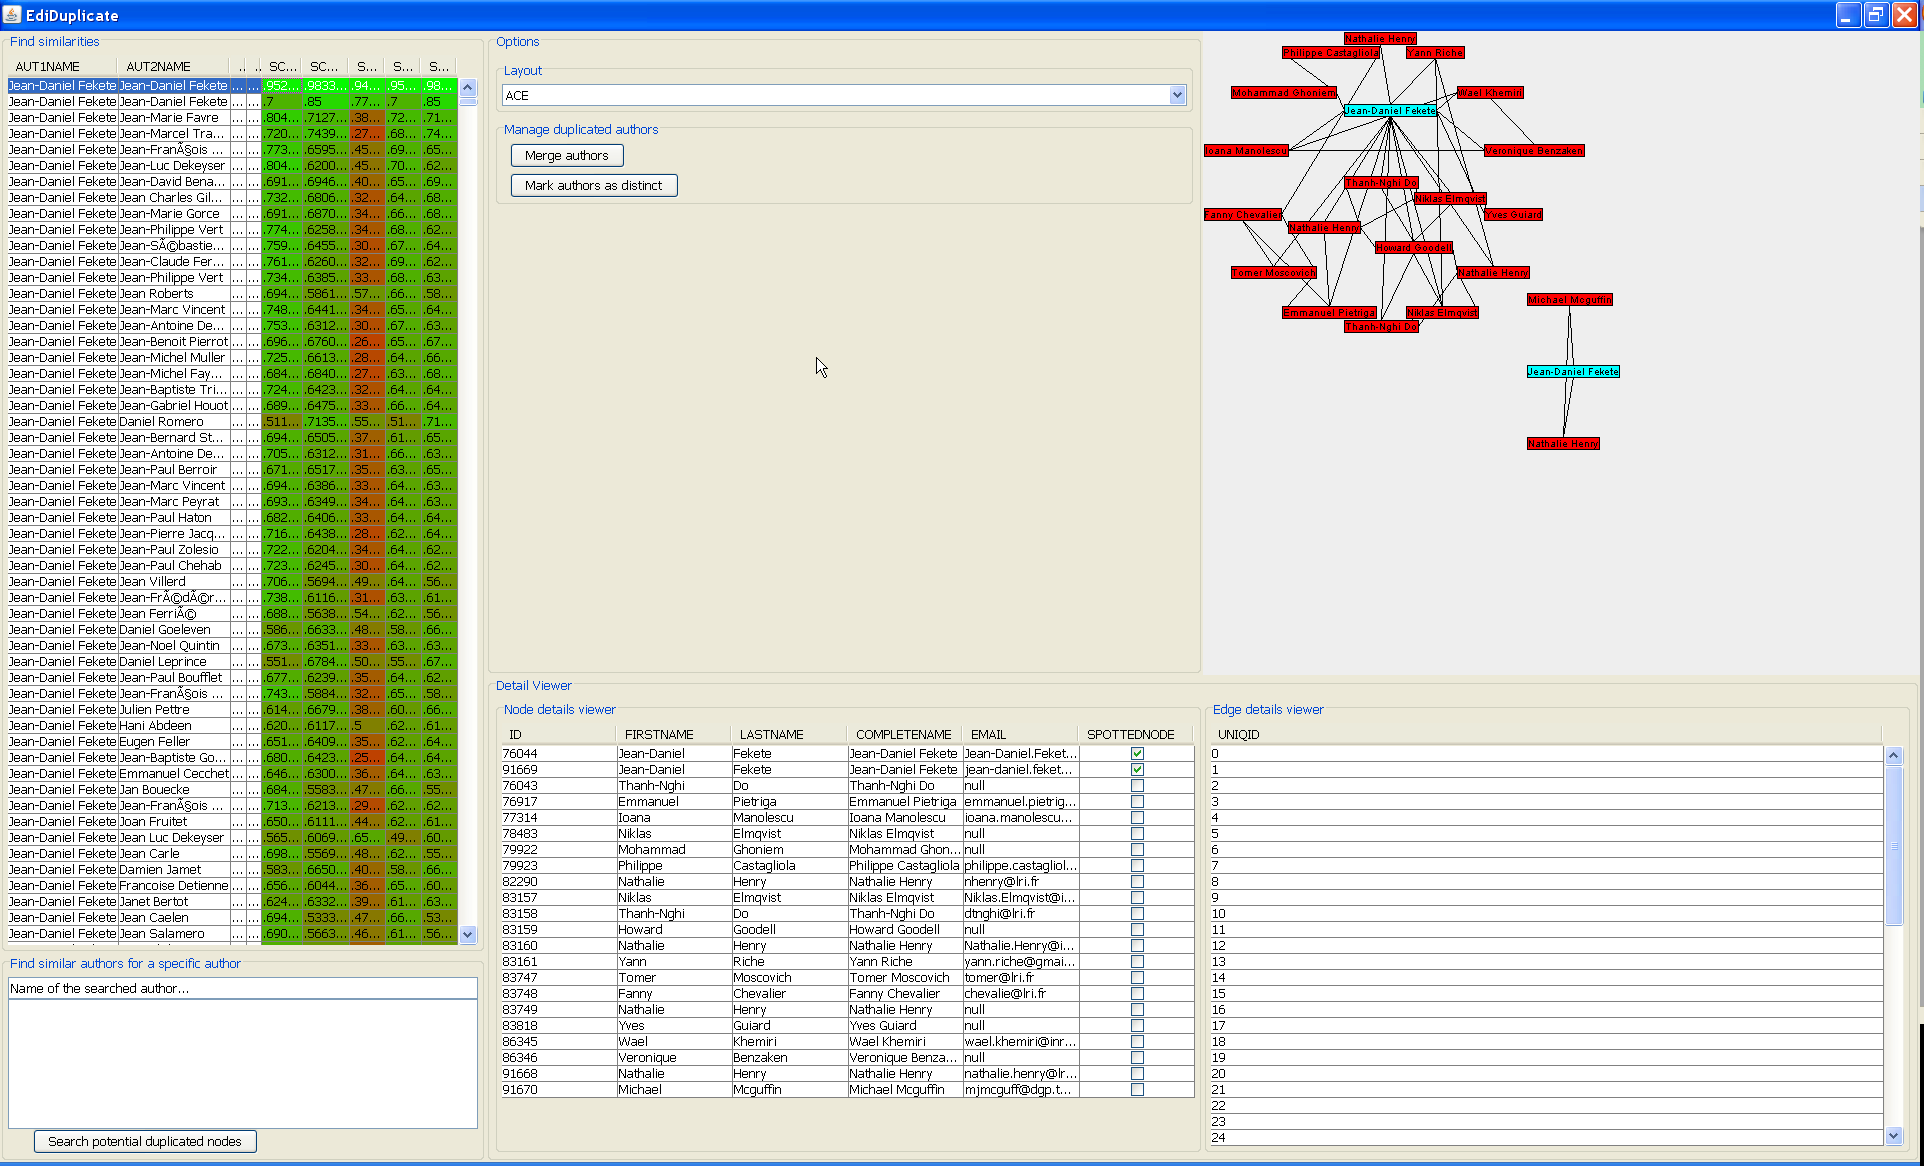
\includegraphics[width=\columnwidth]{figures/ediduplicate}
\caption{A screenshot of Ediduplicate}
\label{fig:ediduplicate}
\end{figure}

EdiDuplicate offers the same possibilities but with extensions to cover specific needs. Concretely, we have implemented a loader to create an Obvious network from the  database. This structure is then fed by an external application with metrics for each pair of authors. Then, those statistics are displayed in a JTable (automically created from the Obvious structure). When, the user clicks on a cell a view of the neighbourhood of the current nodes is created. Then, with this information, the user is able to decide if the potential duplicated authors have to be merged. In addition, it is possible to query the Obvious structure to only display pair of duplicates for a specific authors. The user can also change the layout used to display the neighbourhood network with a JList: all graph layouts introduced in Infovis Toolkit are available. 

Concretely, the application mainly combines Obvious components and Swing components (derived from Obvious structure). For the data model, an Obvious Network is used from the InfoVis Toolkit implementation of Obvious, the visualization and the view part are also provided by this implementation. Building this application takes about less than a week.
\subsection{Implementing a cross-toolkit layout component}

Some of us have tested a potentially important usage scenario: devising a novel layout algorithm and using the Ovious toolkit to make it available in a variety of toolkits. This layout component is a generalized treemap algorithm.
% ~\cite{Treemaps2011}. 
Its interface makes it easy to port as this algorithm takes as input a data model and renders using a Visitor design pattern accross a renderer, making it very convenient to implement accross polyglyphic toolkits like prefuse or Discovery. Considering the current visualization model is mostly targeted at enabling monoglyphic patterns, Obvious in its current state turns out to be of limited use for our purpose.

Still, we have found that the existing data model and utilities have made developing our layout algorithm on top of Obvious worthwhile: we could implement very easily a simple monoglyphic visualization and view instances, and relying on the default data model already saves us time in the development of our prototype, while we have the assurance that only minimal work may be needed to port our method to the toolkits targeted by Obvious.
